\chapter{The LHC and the ATLAS Detector}
\label{sec:det}

\section{The Large Hadron Collider (LHC)}
\label{sec:det-LHC}

High-energy particle colliders have been an essential tool in high-energy physics research for over 50 years,
with a rich history of discovering new particles as each generation of collider pushes the energy frontier;
including the discovery of the Z and W bosons using the Super Proton Synchotron at CERN in 1983~\cite{det-Wdisc_UA1, det-Zdisc_UA1, det-Wdisc_UA2, det-Zdisc_UA2} 
and the discovery of the  top-quark at the Tevatron in 1995~\cite{det-tdisc_CDF, det-tdisc_D0}.

The Large Hadron Collider (LHC) is the highest energy collider ever built,
operated by the \textit{Conseil Europ\'een pour la Recherche Nucl\'eaire (CERN)}.
Lying in a tunnel \SI{100}{\metre} beneath the Swiss/French border near Geneva,
the LHC is a \SI{27}{\km} circumference ring of superconducting magnets and accelerating structures,
which accelerate beams of protons to a maximum energy of \SI{6.5}{\TeV}.
These proton beams are collided in four different locations on the LHC ring
and around each collision point a different detector is constructed to observe these collisions;
one such of these detectors is the ATLAS detector.

\subsection{LHC running conditions in 2015 and 2016}

Since May 2015 the LHC has been colliding bunches of protons at a center-of-mass energy of \SI{13}{\TeV},
the highest energy collisions ever obtained by a particle collider
\footnote{The period of data-taking from 2015 is known as Run-2.}.
In 2015 and 2016 the LHC produced $pp$ collisions 
with a bunch spacing of \SI{25}{\nano\second}\footnote{A small amount of data in 2015 was collected with a bunch spacing of \SI{50}{\nano\second}}

\textit{Integrated luminosity}, $L$, is the quantity used to describe the size of a data-set from a collider experiment.
Integrated luminosity is defined is defined using $N_{evt} = \sigma * L$,
where $\sigma$ is the cross-section of a particular process occuring at that collider experiment and $N_{evt}$ is the number of events that occur throught that process in the data-set.
Instantaneous luminosity is the measure used to define the rate of data-collecting by the ATLAS detector and is defined as $\frac{dL}{dt}$.

Figure \ref{fig:det-lumi_2015_2016} shows the integrated luminosity delivered by the LHC and recorded by ATLAS in 2015 and 2016;
an integrated luminosity of \SI{3.9}{\fb^{-1}} and \SI{35.6}{\fb^{-1}} was recorded by ATLAS in 2015 and 2016 respectively~\cite{det-ATLAS_lumi_twiki}.
\begin{figure}[!ht]
  \begin{center}
    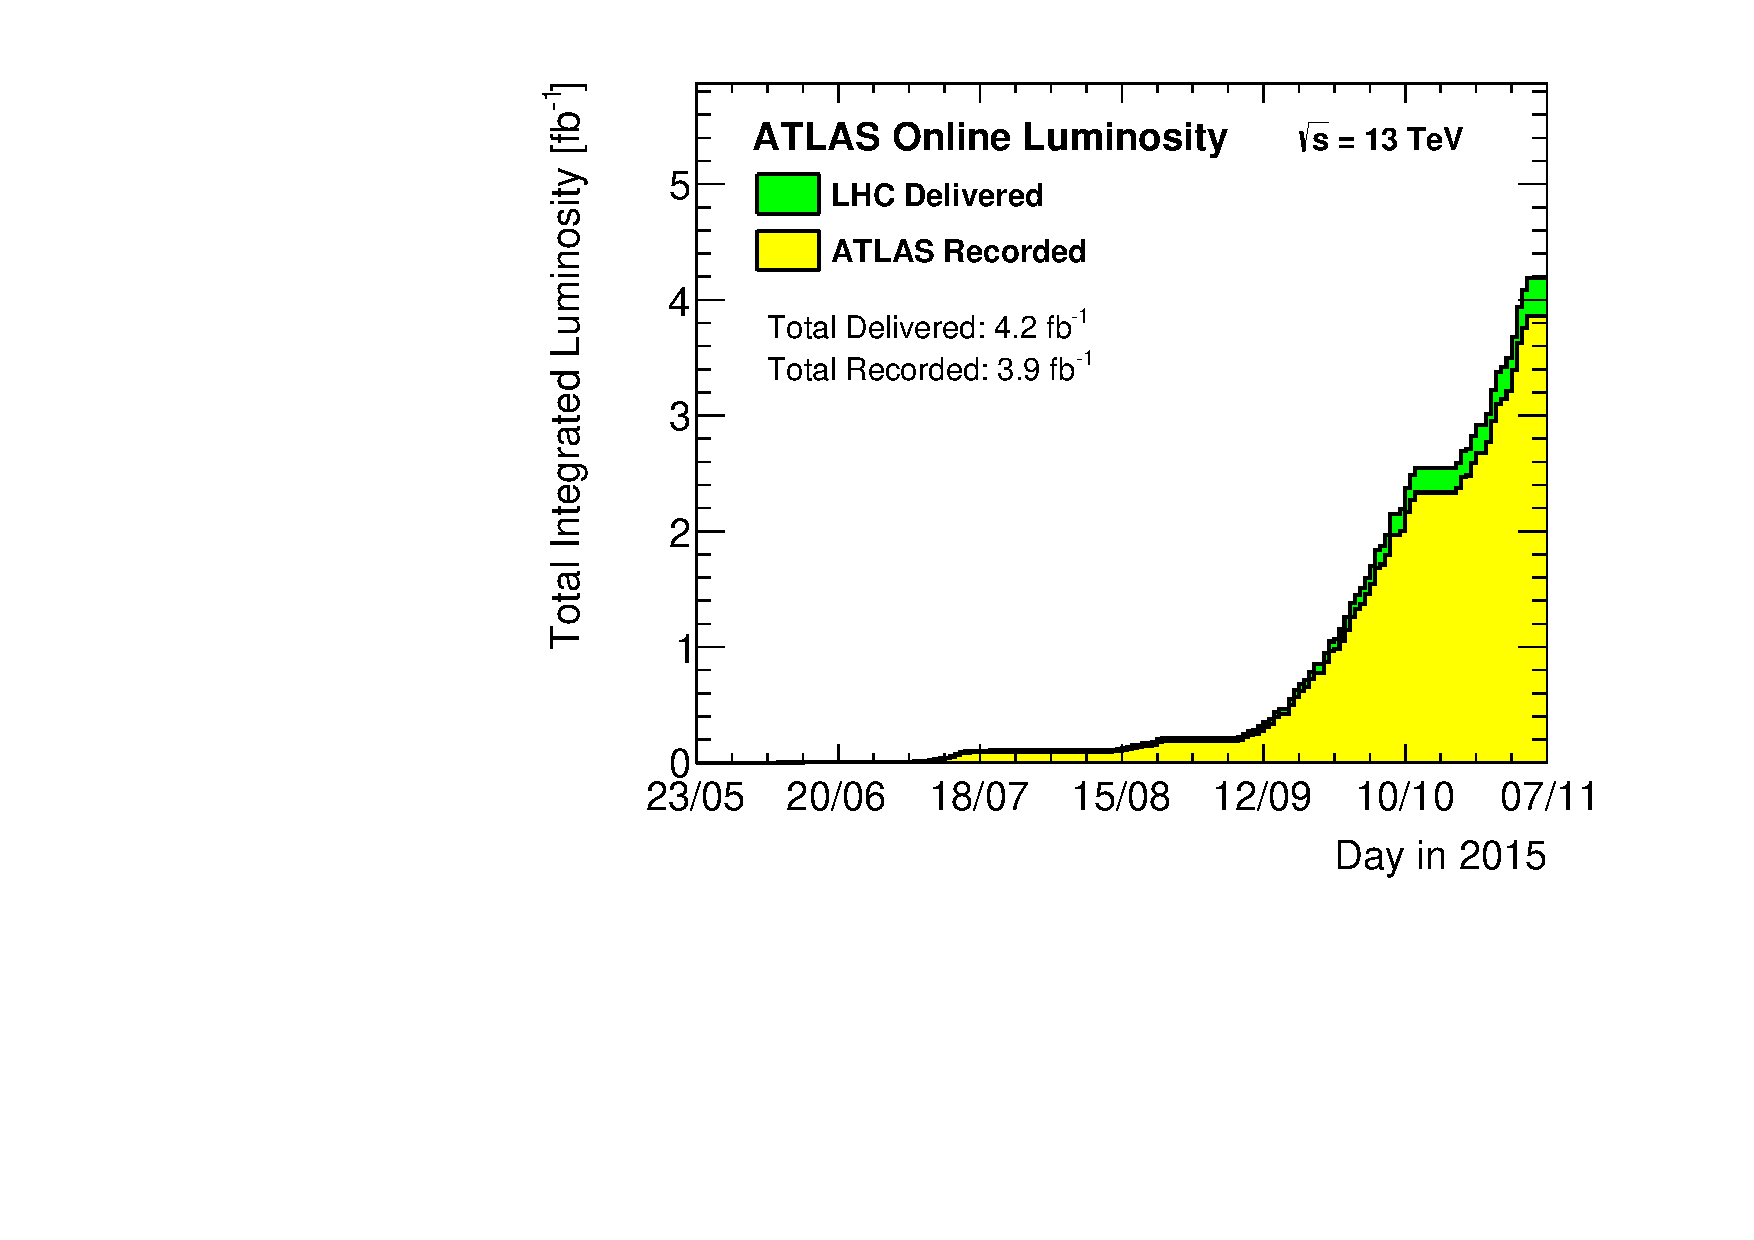
\includegraphics[width=0.45\linewidth, angle=0]{figs/Detector/lumi_2015.pdf}
    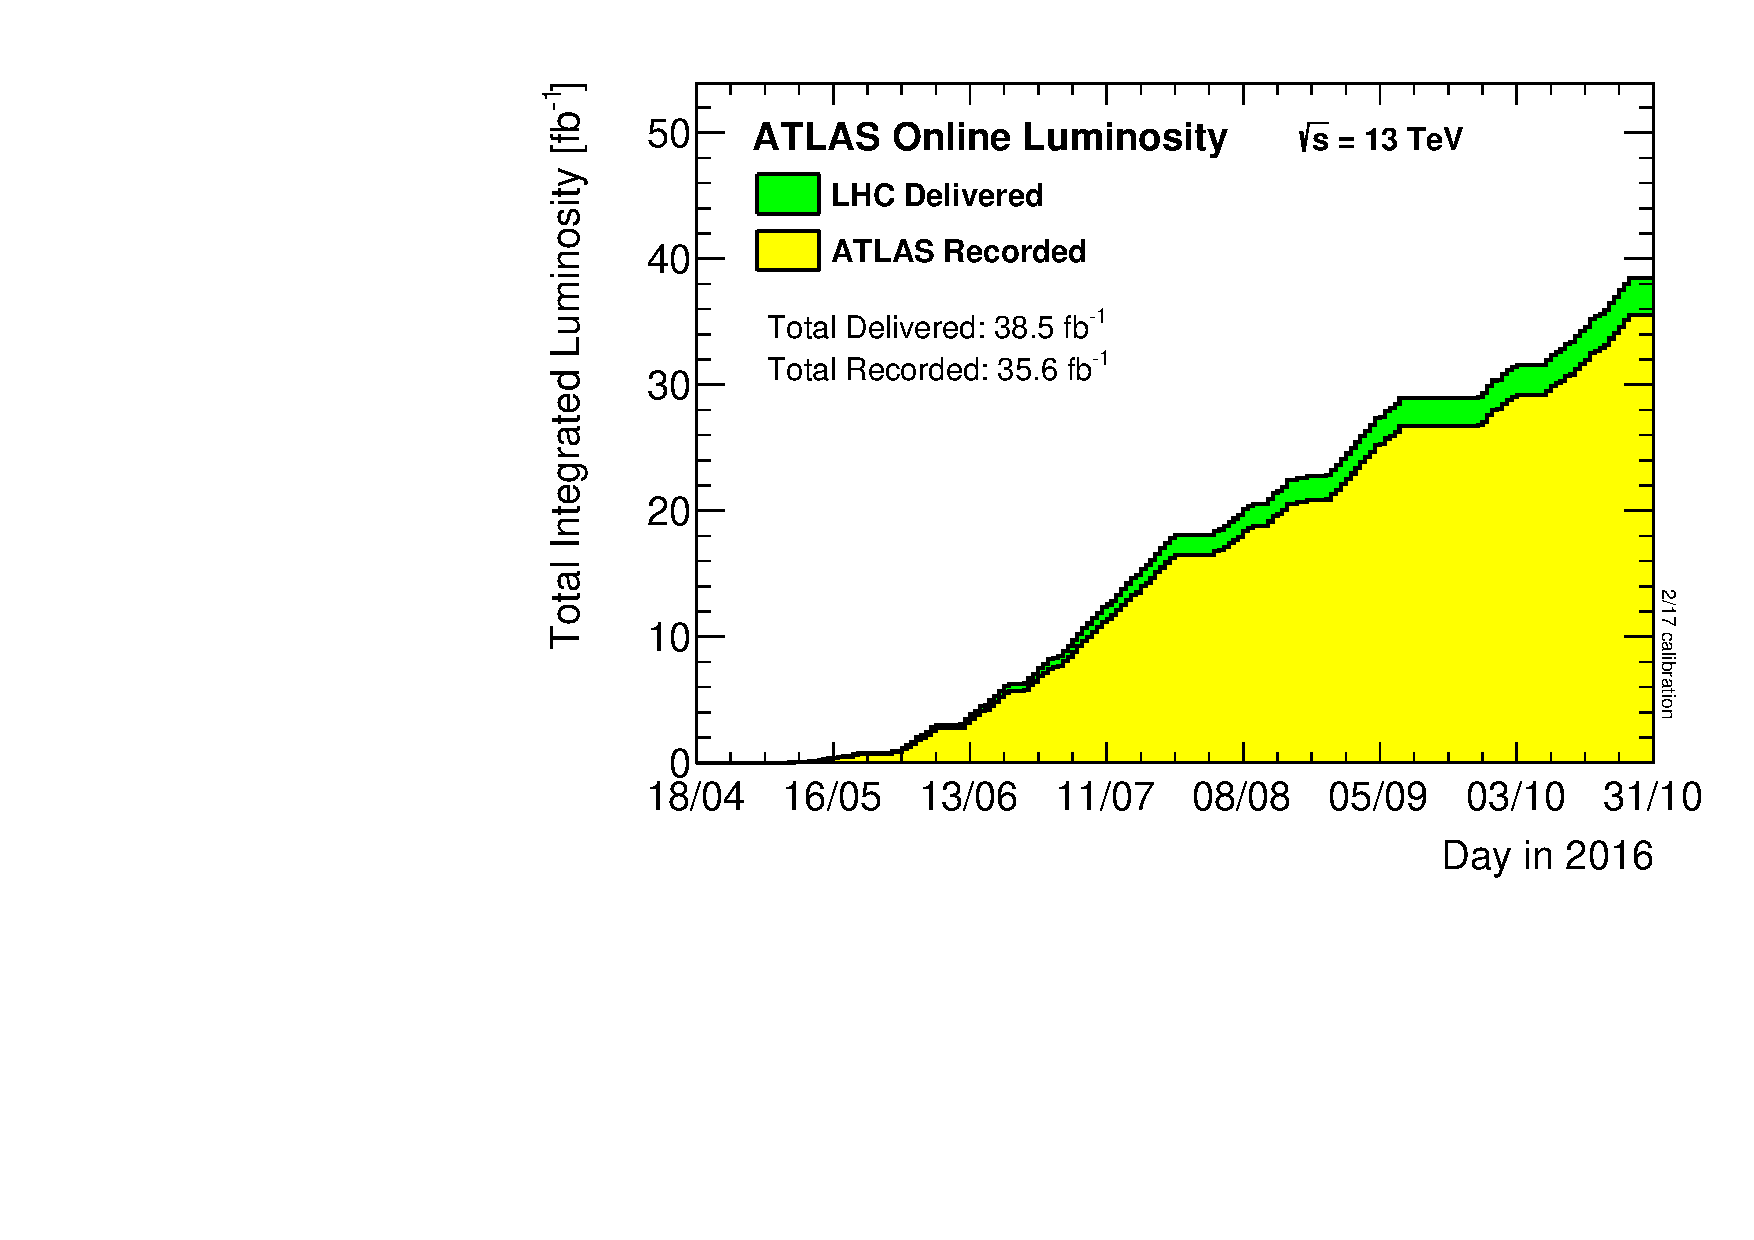
\includegraphics[width=0.45\linewidth, angle=0]{figs/Detector/lumi_2016.pdf}
  \end{center}
  \vspace{-1em}
  \caption[Integrated luminosity versus time delivered to and recorded by ATLAS during 2015 and 2016]
          {  \label{fig:det-lumi_2015_2016} Integrated luminosity versus time delivered to (green) and recorded by ATLAS (yellow) during stable beams for $pp$ collisions
            at 13 TeV centre-of-mass energy \mbox{in (a) 2015 and (b) 2016~\cite{det-ATLAS_lumi_twiki}}.}
\end{figure}

To be able to produce a high instantanous luminosity bunches of protons are collided meaning that there is more than one collision per bunch-crossing.
This causes \textit{`pile-up'} to occur;
which is physics objects caused by collisions other than the hard-scatter collision \footnote{Hard-scatter refers a collision that produced a high-\pT object} of interest.
The average number of collisions per bunch-crossing ($<\hspace{-3pt}\mu\hspace{-3pt}>$) is 23.7 in 2015 and 2016 data taken by ATLAS.

\section{ATLAS Detector Description}
\label{sec:det-ATLAS}

The ATLAS (\textbf{A} \textbf{T}oroidal \textbf{L}arge Hadron Collider \textbf{A}pparatu\textbf{S}) detector
design, construction and performance has been described in detail in~\cite{det-ATLAS_Exp, det-ATLAS_TDR, det-ATLAS_Perf}.
Therefore this chapter provides a general description of the detector with a focus on the needs of di-$b$-jet searches.

The ATLAS detector is effectively a large closed cylindrical detector,
made up of four key components which sit in concentric rings around the interaction point, where the proton bunches collide.
These components are the inner detector, calorimeters, muon spectrometer and the magnets; each of which are described in further detail below.
This design is used as each sub-detector measures different quantities and interacts differently to the various range of particles that ATLAS is required to observe,
such that the ATLAS detector is able to identify and measure the key properties \footnote{\ For example four-momentum and charge.}
of particles that pass through its volume.
Figure~\ref{fig:det-ATLAS_schem} shows a cut-away schematic of the detector
and Figure~\ref{fig:det-ATLAS_slice} shows a slice of the detector in the plane perpendicular to the beam-pipe,
overlaid are simplified illustrations how the detector responds to a range of particles~\cite{det-thesis_gutchow}.


\begin{figure}[!ht]
  \begin{center}
    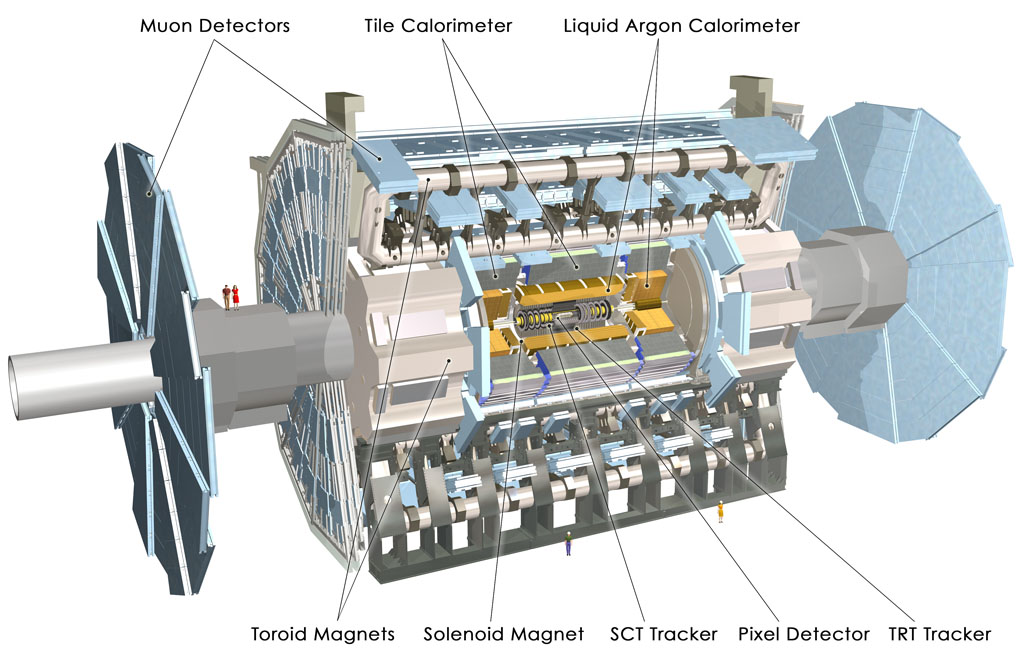
\includegraphics[width=1\linewidth, angle=0]{figs/Detector/ATLAS_schem.jpg}
  \end{center}
  \caption[A cut-away schematic of the ATLAS detector.]{ A cut-away schematic of the ATLAS detector~\cite{det-ATLAS_Exp}.}
  \label{fig:det-ATLAS_schem}
\end{figure}
\begin{figure}[!ht]
  \begin{center}
    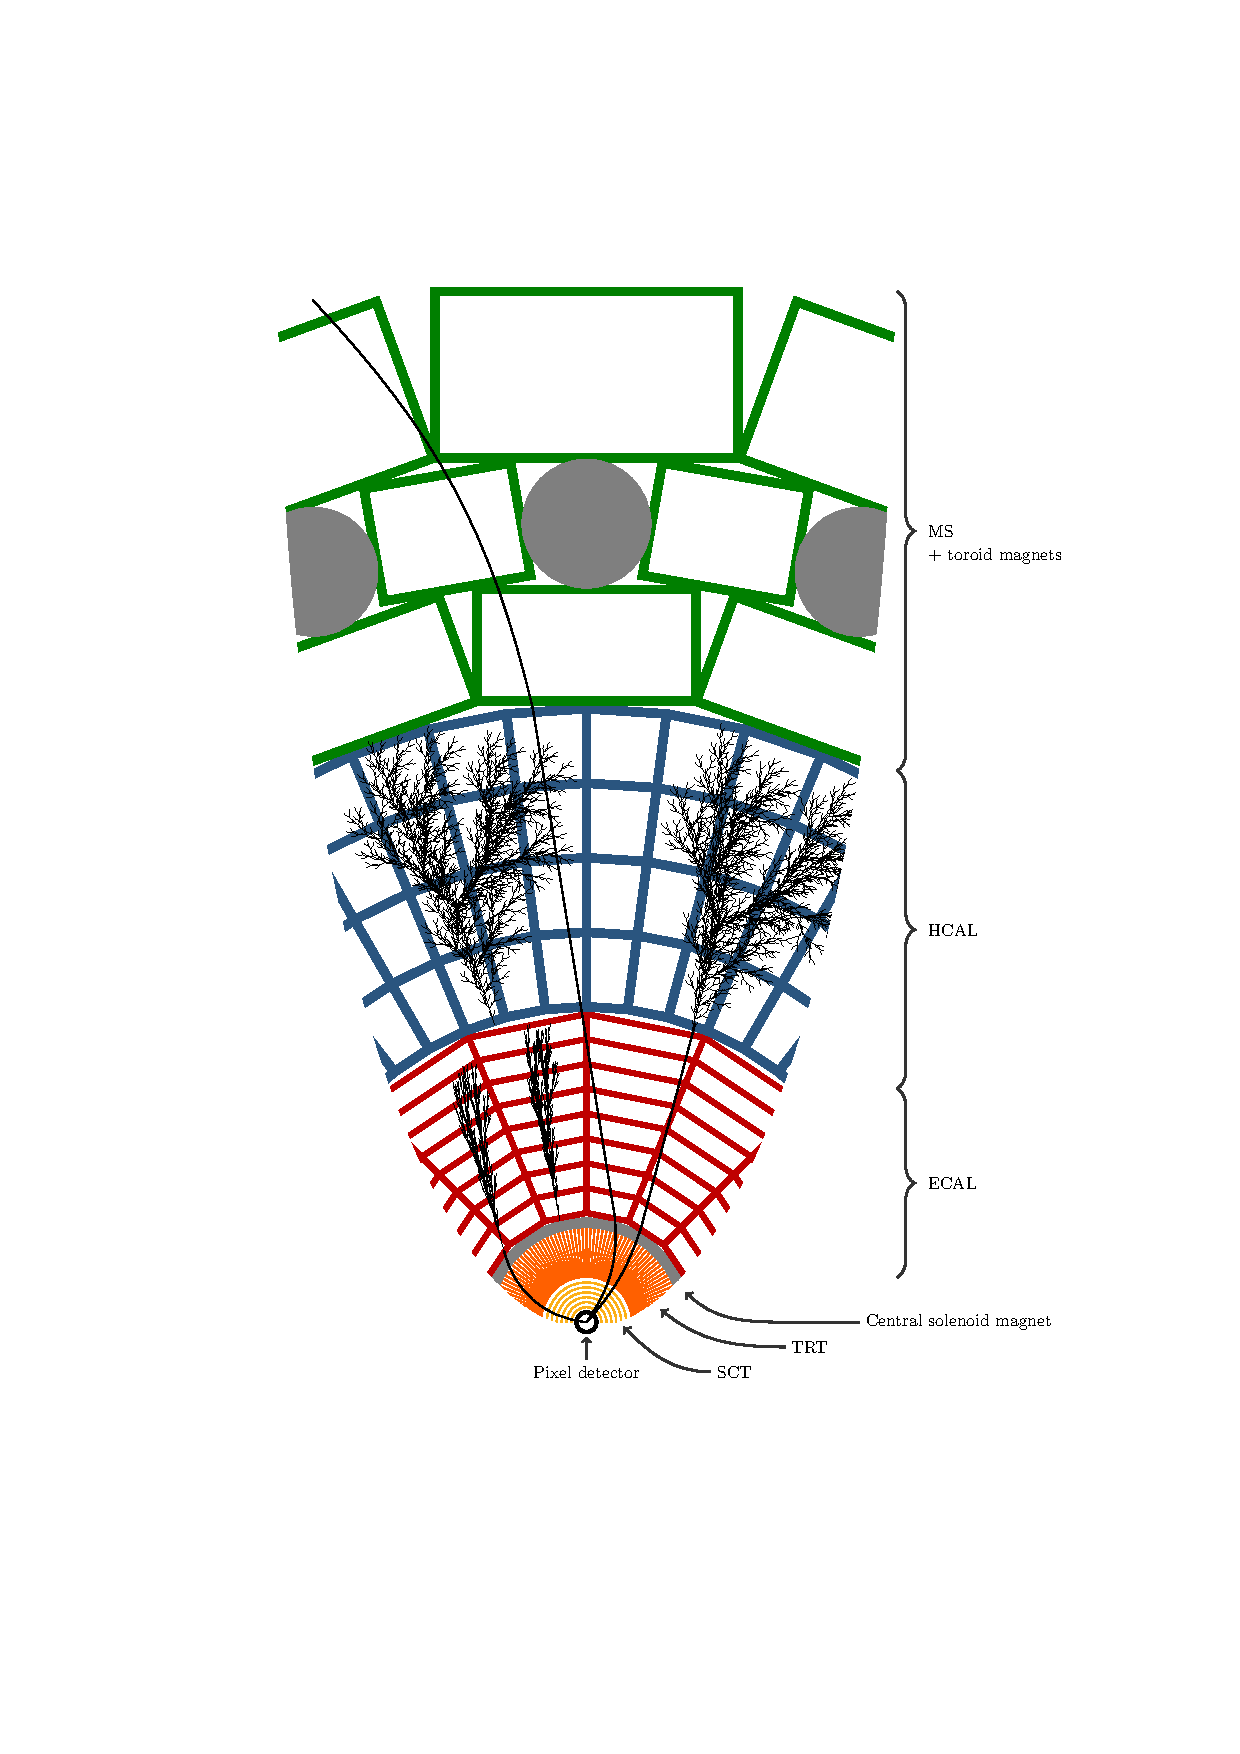
\includegraphics[width=0.7\linewidth, angle=0]{figs/Detector/ATLAS_slice.pdf}
  \end{center}
  %When citing in a caption, use this set-up
  \caption[A visualisation of the ATLAS detector and the various sub-detectors with simplified illustrations of how various types of particles interact with the ATLAS detector overlaid.]
          {A visualisation of the ATLAS detector and the various sub-detectors.
    The view is taken as a slice in a plane perpendicular to the beam-pipe,
    showing the radial range from the beam-pipe to the edge of the detector.
    Overlaid are simplified illustrations of how various types of particles interact with the ATLAS detector;
    specifically from left to right the particles are an electron, a chargeless hadron (e.g. a neutron), a photon, a muon and a charged hadron (e.g. proton).
    The sub-detector components are not to scale~\cite{det-thesis_gutchow}.}
  \label{fig:det-ATLAS_slice}
\end{figure}

\subsection{ATLAS Co-ordinate System}
\label{sec:det-coordinate}

Firstly, to describe the detail of the ATLAS detector there must be a description of the co-ordinate system that is used.
ATLAS uses a right-handed coordinate system, in which the origin lies at the interaction point.
The $x$-axis points towards the centre of the LHC ring parallel to the surface of the earth,
the $y$-axis points upwards towards the surface of the earth
and the $z$-axis runs along the beam-pipe, pointing anti-clockwise along the LHC beam-pipe.
The azimuthal angle, $\phi$, is defined right-handedly around the $z$-axis starting at the $x$-axis.
%Figure~\ref{fig:det_coordinate} illustrates this co-ordinate system.


The polar angle, $\theta$, is defined as the angle measured from the $z$-axis,
such that along the $z$-axis corresponds to $\theta = 0$
and anti-aligned with the $z$-axis corresponds to $\theta = \pi$.
However, to define the angular direction with respect to the z-axis the ATLAS co-ordinate system uses pseudo-rapidity, $\eta$, instead of using \theta, for reasons that will be outlined below.
$\eta$ is defined as a function of $\theta$:
\begin{equation}
 \eta = -\ln\left[\tan\left( \frac{\theta}{2} \right) \right]
\end{equation}
Thus, $\eta = 0$ corresponds to a particle travelling perpendicular to the beam-pipe,
where a positive value of $\eta$ corresponds to a particle travelling with a tilt towards the positive $z$-axis.
The quantity is called pseudo-rapidity as in the massless limit ($\lim_{E\to|\vec{p}|}$)
it can be shown that $\eta$ converges to rapidity, $y$, where rapidity is defined as,
\begin{equation}
  y = \frac{1}{2} \ln \left( \frac{E+p_{z}}{E-p_{z}} \right)
\end{equation}
A key property of rapidity is that differences in rapidity, $\Delta y$, are invariant against Lorentz boosts along the $z$-axis;
This is important as collisions in $pp$ colliders have different Lorentz boosts along the $z$-axis
caused by the effects of the Parton Distribution Functions described in Section~\ref{sec:theo-qcd_pdf}.
Thus, $\eta$ is the final variable chosen in the ATLAS co-ordinate system due to the relation of $\eta$ with both $\theta$ and $y$
and the above mentioned property of $\Delta y$.

\noindent
The final important quantity of the ATLAS co-ordinate system is $\Delta R$, which is defined as
\begin{equation}
  \Delta R = \sqrt{\Delta\eta^{2} + \Delta\phi^{2}}  \label{eqn:det-deltaR}
\end{equation}
\Delta R represents the angular separation between two vectors in the ATLAS co-ordinate system.


%Now that we have discussed the ATLAS co-ordinate system, we can provide a description of the components of the ATLAS detector.

\subsection{Inner Detector}
\label{sec:det-ID}

The Inner Detector (ID), the innermost sub-detector on ATLAS,
measures the trajectory of charged particles passing through the detector.
The ID is constructed from many concentric layers of detector,
and as a charged particle passes through the detector each of the layers provides a position measurement, known as a hit.
Typically a particle passing through the whole Inner Detector at $\eta=0$ will provide 44 hits. % 4+4+36
Using the hits from the many layers the trajectory of the particle is determined;
the measured trajectory is known as a track \footnote{ The procedure used for track reconstruction will be discussed in Section~\ref{sec:obj-tracks}}.
The ID is immersed in a 2~T magnetic field which bends the particle's trajectories;
the sign of the charge and momentum of the particle is inferred from the sign and magnitude of the track's curvature.

The ID is made of three main component parts; the Insertable B-Layer (IBL), the pixel detector \footnote{ Often the IBL is considered as part of the pixel detector},
the Semi-Conductor Tracker (SCT) and the Transition Radiation Tracker (TRT), as visualised in Figure~\ref{fig:det-ID_slice}.
The figure also shows the radial positions of each of they layers.
The ID provides hits for tracking in the range $\eta < 2.5$;
to achieve this ID components are organised into the barrel, which are cylinders around the beam-pipe in the central region %\footnote{ Central here means at a low value of $|z|$}
of the detector and the end-caps, which are disks that lie perpendicular to beam-pipe on either end of the barrel.
Figure~\ref{fig:det-ID_schem} shows the layout of the barrel and end-cap components for the pixel, SCT and TRT detectors in one half of the detector.
Table~\ref{tab:det-ID} summarises the key properties of the components of the ID in both the barrel and the end cap.

\begin{figure}[!ht]
  \begin{center}
    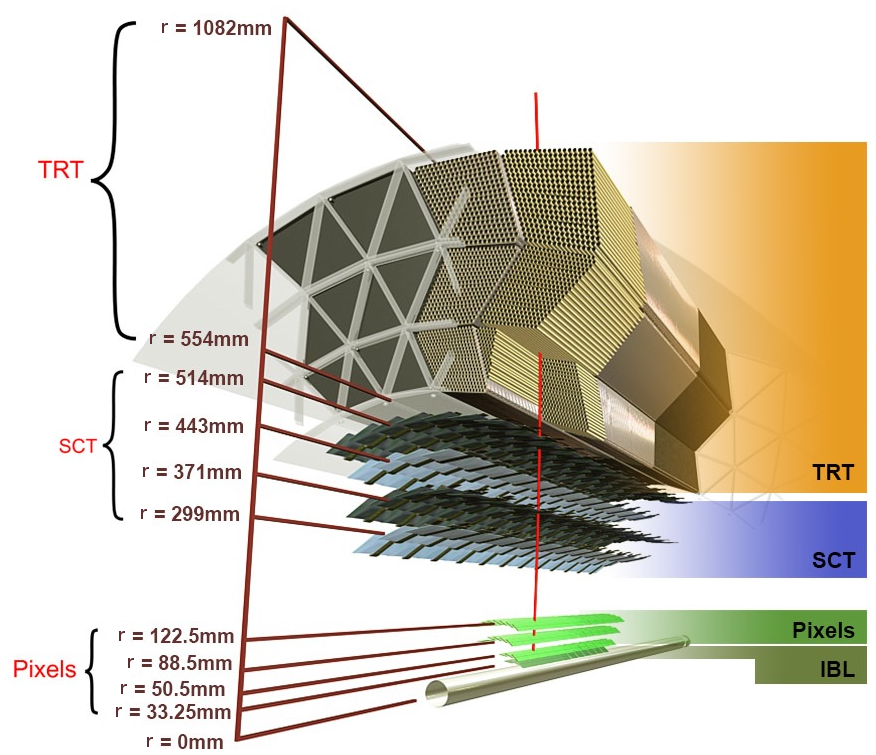
\includegraphics[width=0.8\linewidth, angle=0]{figs/Detector/ID_slice.png}
  \end{center}
  \caption[A schematic showing a slice of the barrel of the ATLAS Inner Detector including the Insertable $B$-Layer.]
          {A schematic showing a slice of the barrel of the ATLAS Inner Detector (ID) including the Insertable $B$-Layer (IBL).
            Each component of the ID is labelled and the radial distances from the beam-pipe ($r$) are shown~\cite{obj-tracks_TIDE}.}
  \label{fig:det-ID_slice}
\end{figure}

\begin{figure}[!ht]
  \begin{center}
    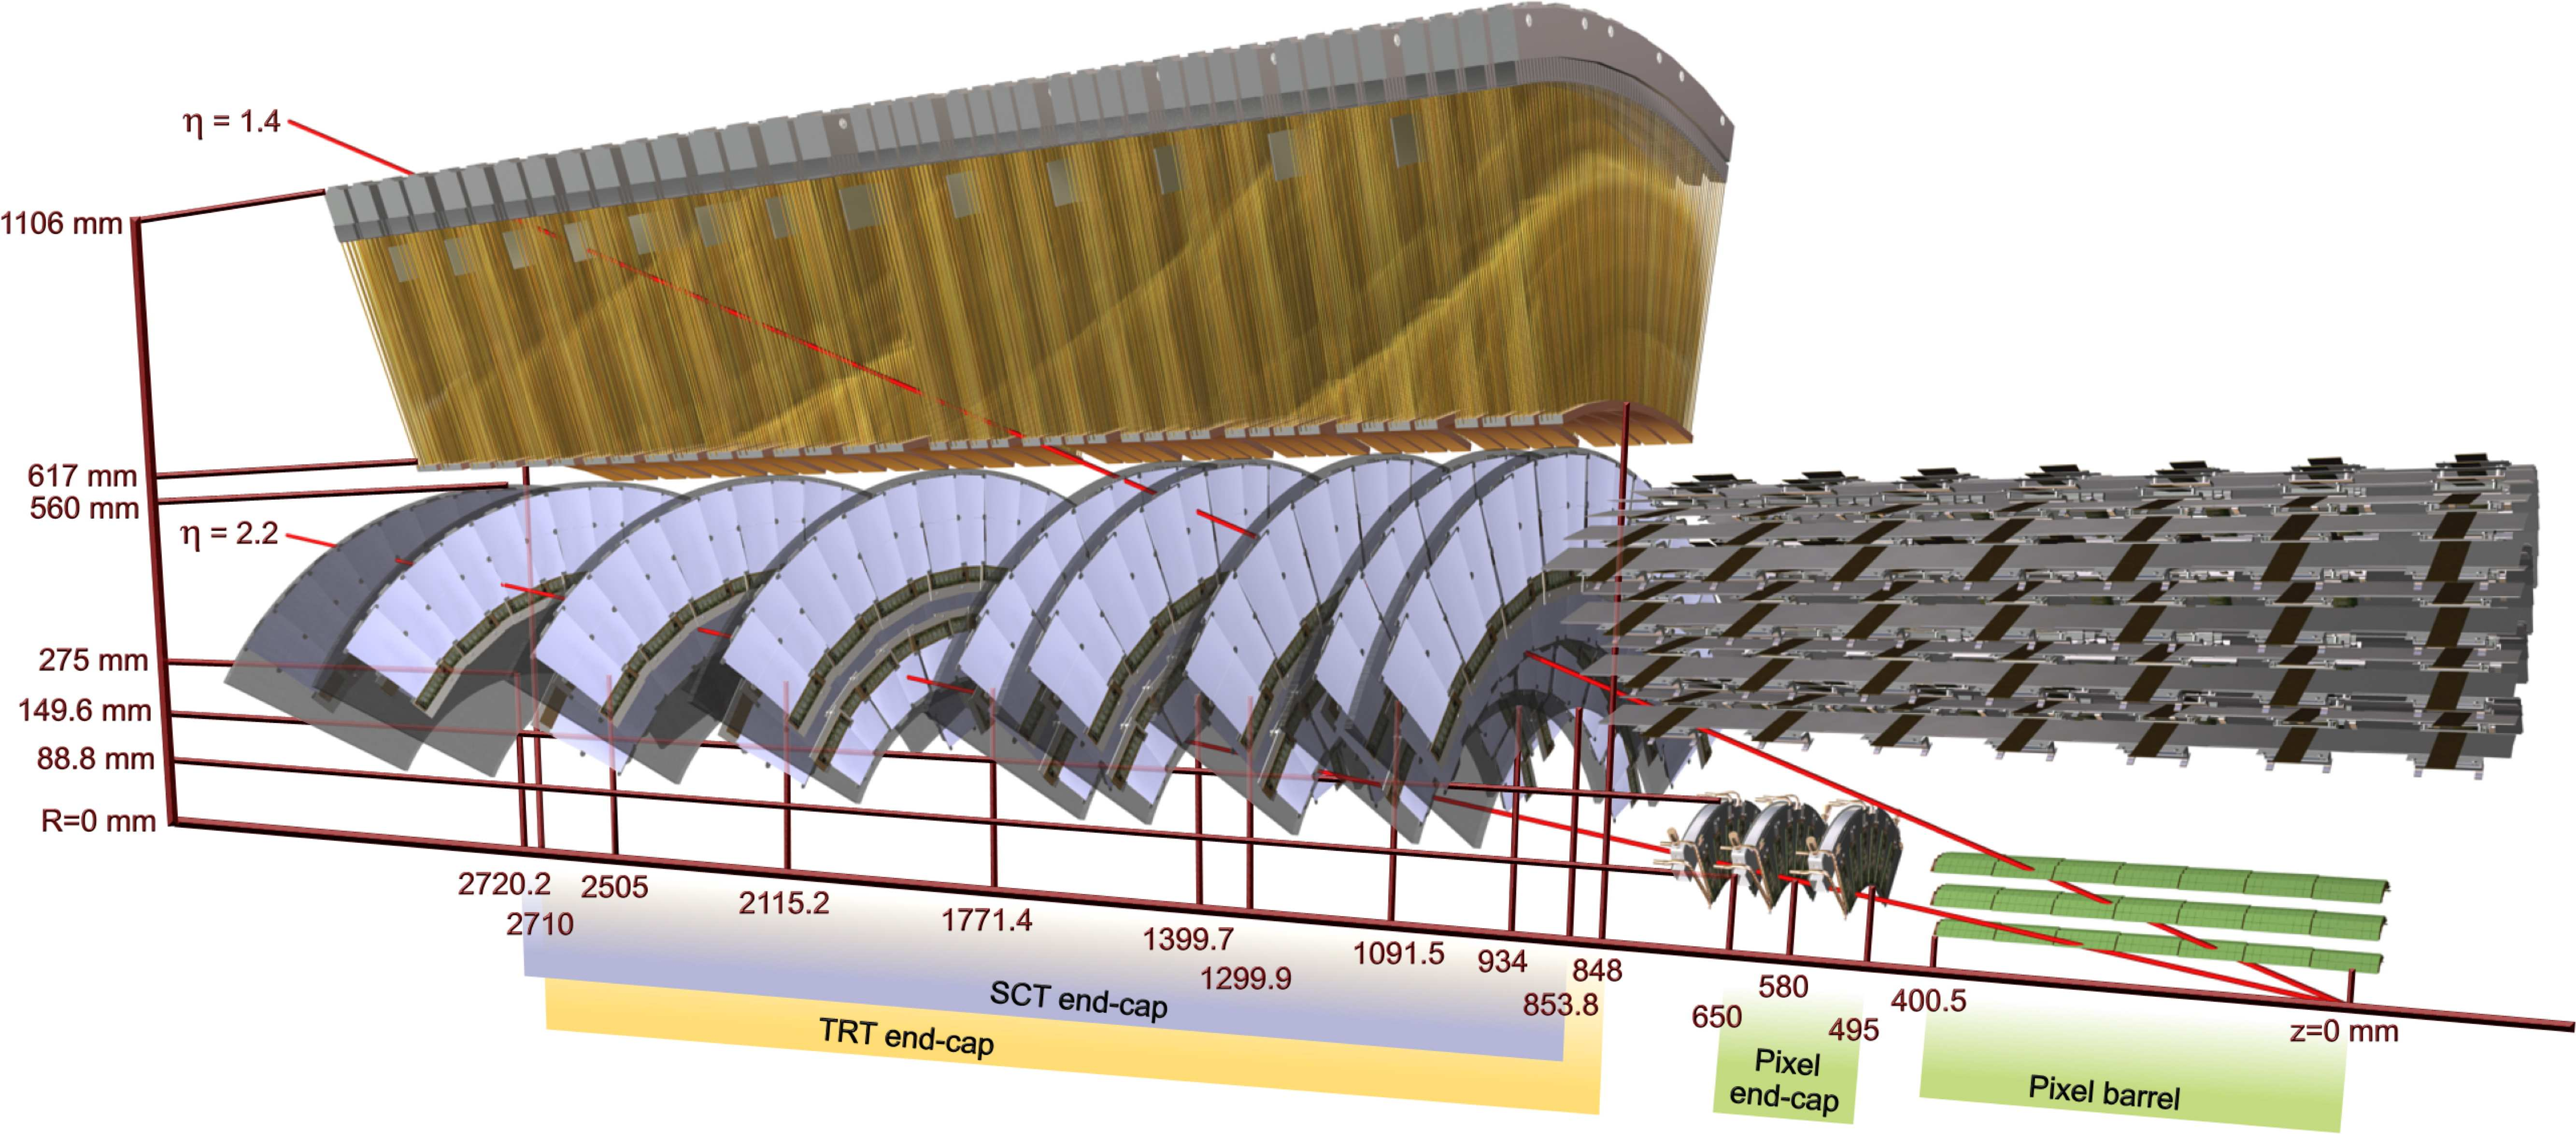
\includegraphics[width=1\linewidth, angle=0]{figs/Detector/ID_schem.pdf}
  \end{center}
  \caption[A schematic showing the barrel and end-cap components of the ATLAS Inner Detector.]
          {A schematic showing the barrel and end-cap components of the ATLAS Inner Detector (ID), the Insertable $B$-Layer is not shown.
            Each component of the ID is labelled and the axial distance from the beam-pipe ($z$) is shown.
            The red lines indicate the trajectory of a particle at $\eta$ = 1.4 and 2.2 with $p_T$ = 10 GeV.~\cite{det-ATLAS_Exp}.}
  \label{fig:det-ID_schem}
\end{figure}


%\begin{figure}[!ht]
%  \begin{center}
%    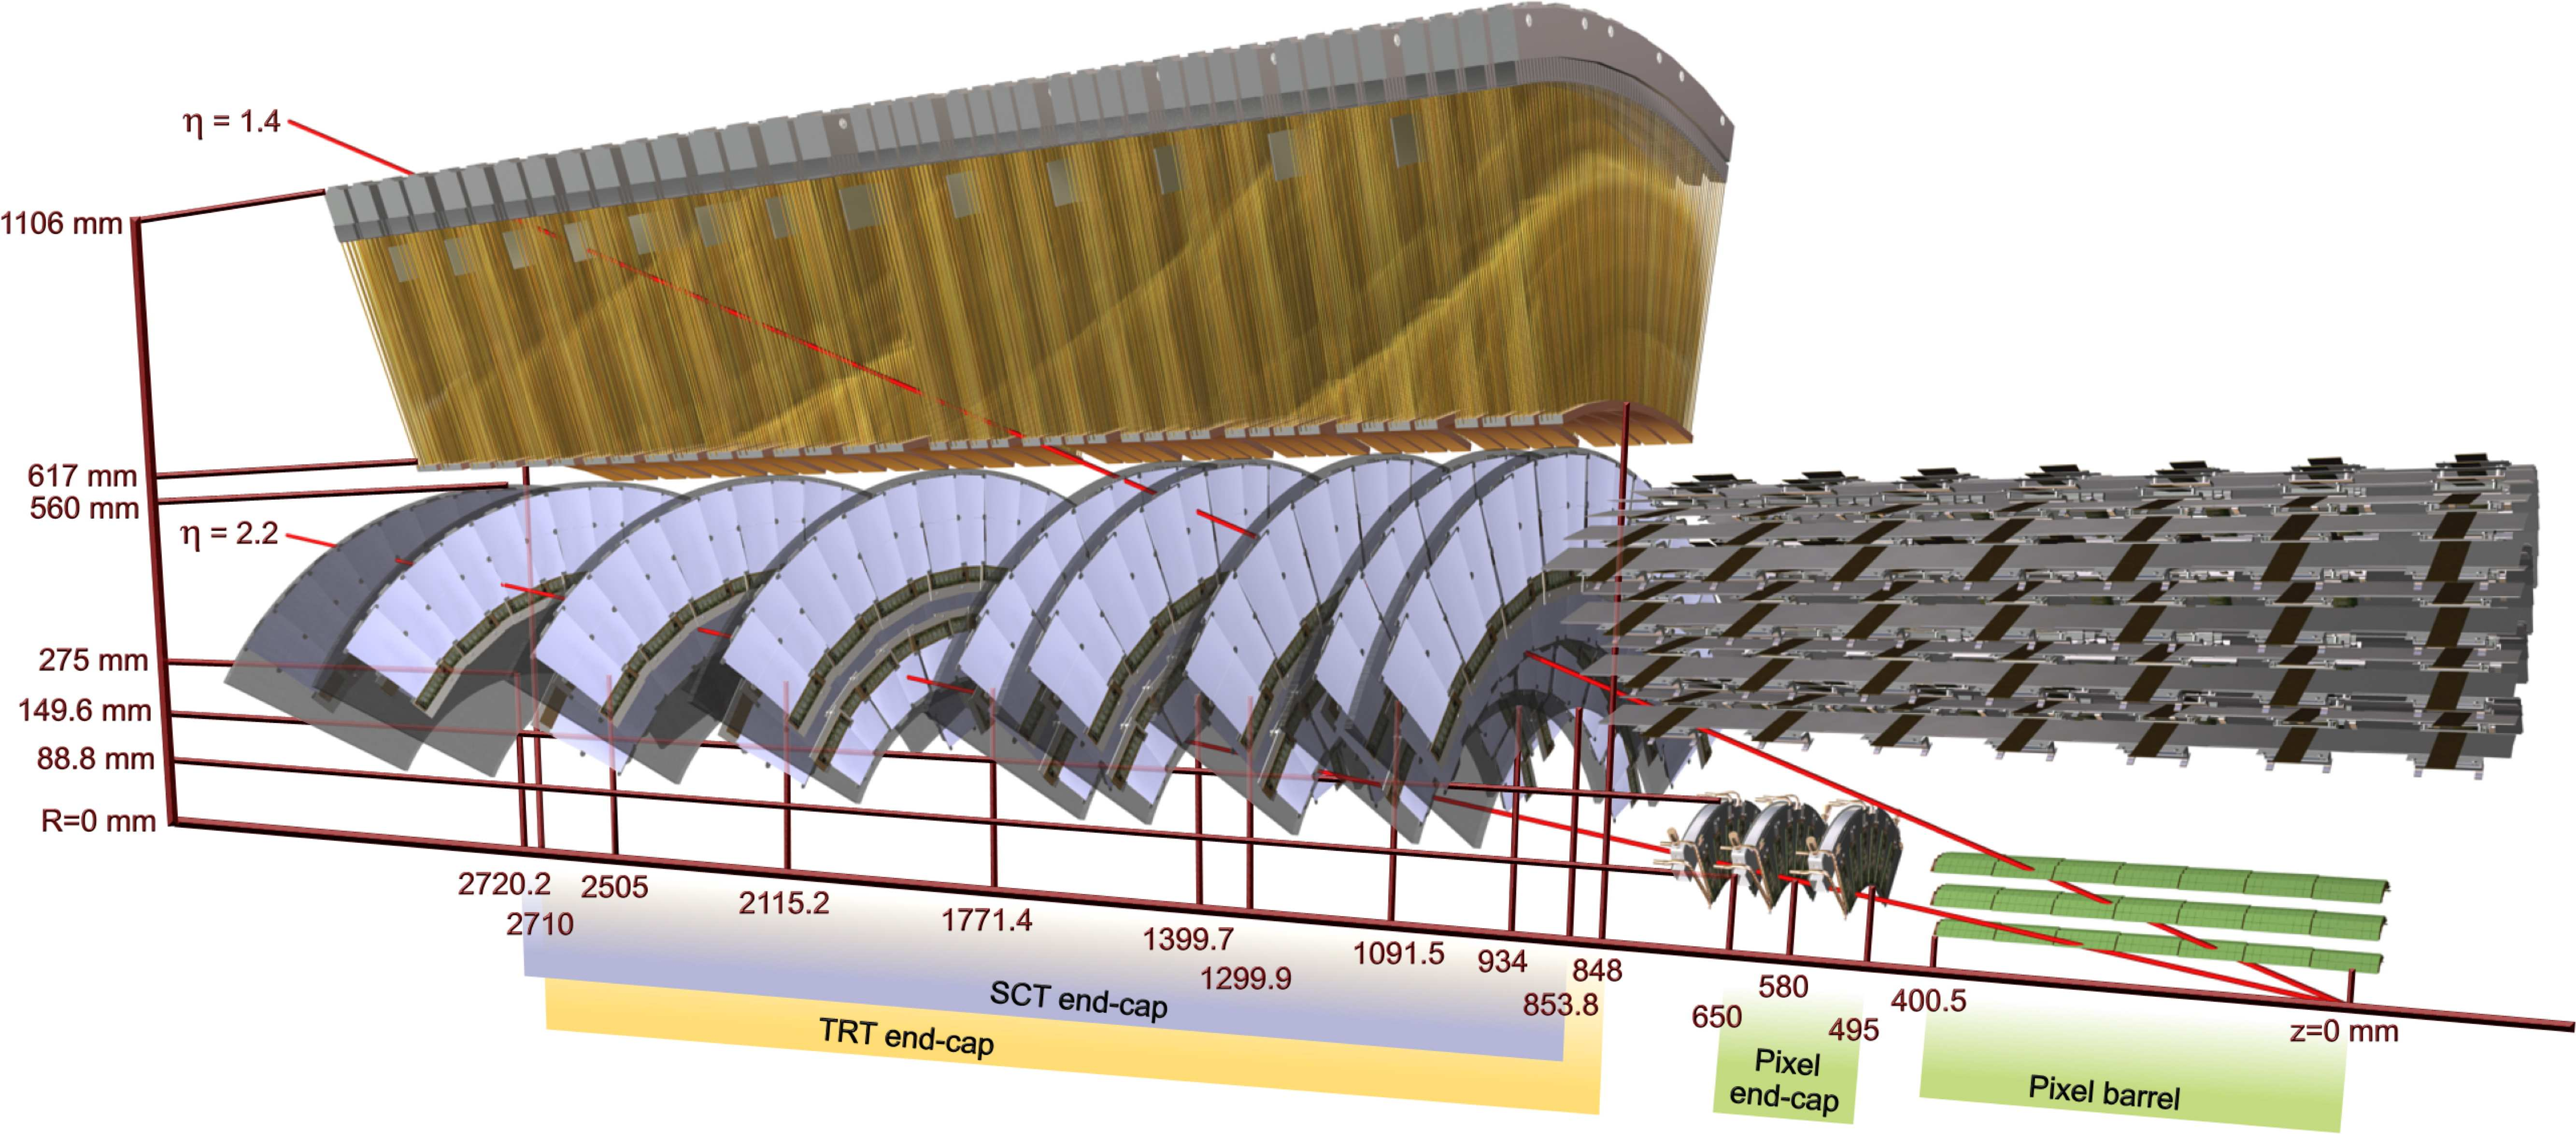
\includegraphics[width=0.8\linewidth, angle=0]{figs/Detector/ID_schem.pdf}
%  \end{center}
%  \caption[A cut-away schematic of the ATLAS Inner Detector (ID).]
%          {A cut-away schematic of the ATLAS Inner Detector (ID)~\cite{det-ATLAS_Exp}.}
%  \label{fig:det-ID_schem}
%\end{figure}

{\renewcommand{\arraystretch}{1.2}
\begin{table}[!htb]
\centering
\begin{tabular}{|cc||c|c|rr|c|}
  \hline
  \multicolumn{2}{|c||}{\textbf{Component}} & \multirow{2}{*}{\textbf{$\eta$ Coverage}} & \textbf{Element} &  \multicolumn{2}{c|}{\textbf{Intrinsic}} & \textbf{\# Layers} \\
  \multicolumn{2}{|c||}{\textbf{of ID}}     &       & \textbf{Size (\SI{}{\micro\metre})}  & \multicolumn{2}{c|}{\textbf{Resolution (\SI{}{\micro\metre})}} &  \textbf{or Disks}          \\
  \hline
  \multirow{2}{*}{\textbf{IBL}} & & \multirow{2}{*}{$|\eta| \lt$  2.5}   & \multirow{2}{*}{50 x 250} & \multirow{2}{*}{8 ($R$-$\phi$)}& \multirow{2}{*}{40 ($z$)}  & \multirow{2}{*}{1} \\ %& 33.25 \\
   &&&&&&\\\hline                                                                                                                                                  
  \multirow{2}{*}{\textbf{Pixel}} & Barrel    &  $|\eta| \lt$  1.7            & \multirow{2}{*}{50 x 400} & 10 ($R$-$\phi$)        & 115 ($z$)          & 3                \\ %& 50.5 -- 122.5    \\
                         & End-cap   &         1.7  $\lt |\eta| \lt$  2.5    &                    & 10 ($R$-$\phi$)        & 115 ($R$)          & 3 (both ends)    \\ %& 88.8 -- 149.6    \\
  \hline                                                                                                                                                
  \multirow{2}{*}{\textbf{SCT}}   & Barrel    & $|\eta| \lt$  1.4             &\multirow{2}{*}{80}       &  17 ($R$-$\phi$)        & 580 ($z$)          & 4                \\ %& 299 -- 514       \\
                         & End-cap   &        1.4  $\lt |\eta| \lt$  2.5    &                   &  17 ($R$-$\phi$)        & 580 ($R$)          & 9 (both ends)    \\ %& 275 -- 560       \\
  \hline                                                                                                                                                
  \multirow{2}{*}{\textbf{TRT}}   & Barrel    & $|\eta| \lt$  0.7             & \multirow{2}{*}{4000}     & \multicolumn{2}{c|}{\multirow{2}{*}{130 ($R$-$\phi$)}}     & $\sim$ 36 hits    \\ %& 563 -- 1066      \\
                         & End-cap   &         0.7  $\lt |\eta| \lt$  2.0    &                  &                         &                  & per track        \\ %& 644 -- 1004     \\
  \hline
\end{tabular}
\caption[Summary of the main characteristics of the components of the ATLAS Inner Detector.]
        {Summary of the main characteristics of the components of the ATLAS Inner Detector~(ID). For the SCT and TRT the element sizes refer to the spacing of the readout strips and the diameter of the straw tubes respectively~\cite{det-ATLAS_Exp,det-ID_table}.}
\label{tab:det-ID}
\end{table}
}


The inner most part of the detector is the Insertable B-Layer (IBL) and the silicon pixel detector,
which are both made out silicon based pixel modules.
The high-granularity of the IBL and pixel detector allow for high precision position measurements (see Table~\ref{tab:det-ID}),
close to the beam pipe, which is important for vertex reconstruction \footnote{ A vertex is defined as the point at which one or more tracks cross}.
The pixel detector is made out of 3 layers in the barrel and 3 end-caps at either end.
The IBL was added to the ID in 2014 to improve tracking efficency,
which had been degeredated by damage to the other layers of the pixel detector cause by data-taking before 2014,
and to provide an extra measurement close to the beam-pipe for improved vertex reconstruction.
The IBL is made out of 1 layer of pixel modules in the barrel only, as this can provide an angular coverage of $\eta <$ 2.5.


Moving radial outwards the next component of the ID is the Semi-Conductor Tracker.
SCT modules are made from paris of semi-conducting strips;
the strips are $\sim$\SI{120}{\mm} in length \footnote{ This number varies for the various parts of the SCT},
have a strip  (spacial seperation between strips) is \SI{80}{\micro\metre}
and the strips in the pairs have a stereo angle of 40 mrad between them.

The outermost component of the ID is the Transition Radiation Tracker (TRT)
constructed of many \SI{4}{\mm} radius cylindrical tubes filled with a xenon based gas mixture
\footnote{ 70\% Xe, 27\% $\text{CO}_2$ and 3\% $\text{O}_2$~\cite{det-ID_xe}.}
%Xenon is used for its high efficiency to absorb TR photons of typical energy 6–15 keV.
with a anode wire through the central axis.
A charged particle passing through the gas causes ionisation allowing a measurement of its position using drift-time.
Furthermore, the space between straws is filled with polymer fibres (barrel) and foils (endcaps) to create transition radiation,
which is emitted by relativistic charged particles as they pass a boundry between materials with different refractive indicies.
The intensity of the transition radiation is inversley proportional to mass, providing additional information for particle identification. 

The trajectory, momentum and charge measurements provided by the Inner Detector are essential for particle identification in ATLAS.
In particular, the high precision measurements close to the beam-line allow for vertex reconstruction,
which is essential for identification of tracks coming from $B$ or $C$ hadrons, and hence the identification of $b$-jets.
The identification of $b$-jets is important for di-$b$-jet searches and so is discussed further in Section~\ref{sec:obj-bjets}.

\subsection{Calorimeters}
\label{sec:det-calo}

The ATLAS calorimeter, located on the outside of the solenoid magnet surrounding the ID,
is designed to provide an energy measurement of the traversing particles.
The ATLAS calorimeter measures the energy of hadronic jets which is used to calculate the invariant mass of jet pairs, %dijet invariant mass,
which is important in the context of di-$b$-jet searches.

The ATLAS calorimeter consists of two different systems built in concentric rings;
the inner-most is the `Electromagnetic Calorimeter system (ECAL)' used to measure electromagnetic objects such as photons and electrons.
Outside of that is the `Hadronic Calorimeter system (HCAL)' that provides an energy measurement of hadronic objects, such as hadronic jets.
The HCAL consists of the Tile and Hadronic Endcap calorimeters.
Both the ECAL and HCAL have barrel and end-cap components to make energy measurements at a large range of $\eta$ values.
Figure \ref{fig:det-calo_schem} shows a cut-away of the ATLAS calorimeter.

\begin{figure}[!ht]
  \begin{center}
    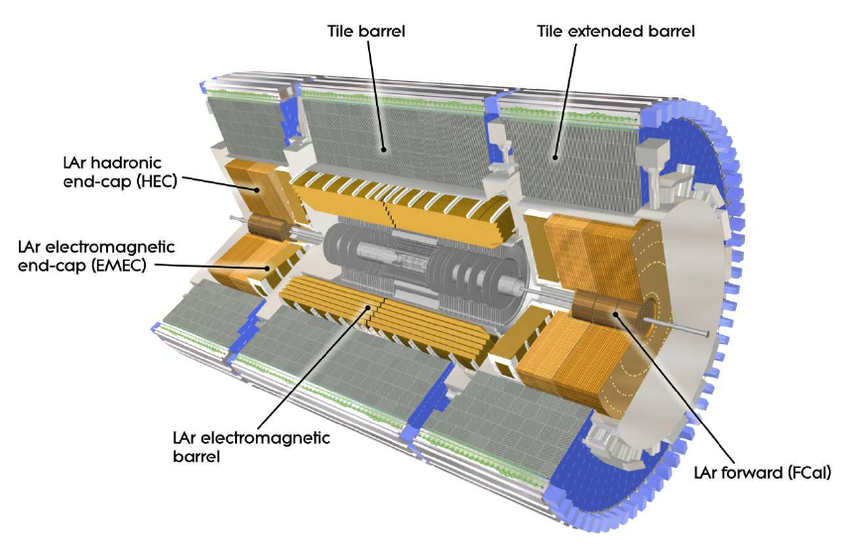
\includegraphics[width=1\linewidth, angle=0]{figs/Detector/Calo_schem.png}
  \end{center}
  \caption[A cut-away schematic of the ATLAS calorimeter system.]
          {A cut-away schematic of the ATLAS calorimeter system~\cite{det-ATLAS_Exp}.}
  \label{fig:det-calo_schem}
\end{figure}

A more detailed description of each of the calorimeter components will follow;
however, the principle behind each detector is common so is described first.
The calorimeters at ATLAS are sampling calorimeters, which means they consist of alternating layers of absorber and active material.
The role of the \textit{`absorber layer'} is to force the particle, whose energy we want to measure, to emit secondary particles.
These secondary particles will again emit further particles and so on meaning a `particle cascade' is formed,
the many resulting particles from the cascade are known as the cascade particles.
The role of the \textit{`active material layer'} is to measure the energy of the many resulting particles from the cascade,
the techniques used by active layers in the ECAL and HCAL are different so will be described below.
The ATLAS detector is built such that the initial particle will fully cascade within the volume of the calorimeter system
and then, from the sum of the energy of the cascade particles, the energy of the initial particle is inferred. 

\subsubsection{Electromagnetic Calorimeter (ECAL)}

For the electromagnetic interaction, at energies above the critical energy of a material ($\sim$\SI{7}{\MeV} for Lead~\cite{obj-bjets_PDG})
the particle cascade process is dominated by two processes;
bremsstrahlung, ($e^{\pm} \to e^{\pm} + \gamma$) and pair production ($\gamma \to e^{+} + e^{-}$).
The electromagnetic calorimeter at ATLAS is known as the `Liquid Argon (LAr) calorimeter'.
The absorber material used in the LAr calorimeter is lead, due to its large density of charged particles (high Z)
which increases the rate of the cascade processes.
The active material is liquid argon (LAr);
when a cascade particle passes through the liquid argon it causes ionisation, and the released electrons are captured and counted using an electric field.
Ionisation dominates the cascade process when the cascade particles are below the critical energy of a material ($\sim$\SI{30}{\MeV} for LAr)
so the released electrons by ionisation will approximately have a constant mean energy (roughly the critical energy of the material minus the energy required to ionise).
Therefore, the number of released electrons is proportional to the energy of the cascade particle,
meaning that the energy of the cascade particle can be measured. 

As discussed above the LAr calorimeter is split up into two sections;
the barrel section covers a region of $|\eta| < 1.475$ and two end-cap components cover $1.375 < |\eta| < 3.2$.
The depth of an electromagnetic calorimeter is often expressed in units of radiation length, $X_{0}$,
which is both the mean distance that an electron loses all but  $1/e$ of its energy through bremsstrahlung
and 7/9 of the mean free path for a photon to produce an $e^+e^-$ pair.
High-Z materials have a shorter radiation length; in lead $X_0$ = 0.56 cm.
The LAr calorimeter has a depth of $>$ 22 $X_{0}$ in the barrel and $>$ 24 $X_{0}$ in the end-caps,
meaning that almost all of the particle shower from a high-energy photon
or electron is contained within electromagnetic calorimeter.
The maximum granularity of the LAr calorimeter in the $\eta$--$\phi$ plane
is 0.025 x 0.025 for the Barrel and 0.025 x 0.1 for the end-cap
\footnote{Full details on the granularity of all components of the ATLAS calorimeter is found in Table 1.3 of~\cite{det-ATLAS_Exp}.}. 

\subsubsection{Hadronic Calorimeter (HCAL)}
\label{sec:det-calo_HCAL}

For particles that interact throught the strong force, such as the components of a hadronic jet,
the particle cascade is a more complicated process.
A hadronic cascade is dominated by processes such as
ionisation, nuclear spallation and neutron generation \cite{det-nuclearInt_book, det-thesis_kate}.
For a chargeless hadron, for example a neutron,
strong processes, such as spallation, are the only processes that contribute to its cascade.
During these hadronic cascade processes many $\pi_0$ mesons are created,
which can decay to a pair of photons and thus form electromagnetic cascade, as described above. 

For hadronic interactions, the depth of detector is given in units of the interaction length, $\lambda$,
defined as the distance required to reduce the number of relativistic hadrons by $1/e$.

By the end of the LAr calorimeter there is 2.3 $\lambda$ of active material in the barrel.
This means that hadronic shower depth is larger than the depth of the LAr calorimeter,
therefore for a full measurement of the hadronic energy, the Hadronic Calorimeter system (HCAL) is required. 

The Tile Calorimeter is constructed from absorber layers of steel and active material layers of scintillating tiles.
The cascade particles produced by the absorber will excite atoms in the scintilating tiles which will then produce photons at a constant mean energy,
therefore by measuring the intensity of the scintilating light (number of photons produced) the energy of the cascade particle can be determined.
The Tile Calorimeter has a depth of 7.4 $\lambda$, meaning the majority of the hadronic shower is captured by the LAr and Tile calorimeter.
The Tile Calorimeter is split up into the barrel and the extended barrel components;
the barrel covers the region $|\eta| <$ 1.0 and the extended barrel covers the region $0.8 < |\eta| < 1.7$.
The maximum granularity of the Tile calorimeter in the $\eta$--$\phi$ plane
is 0.1 x 0.1 for both the barrel and the extended barrel
\footnote{Full details on the granularity of all components of the ATLAS calorimeter is found in Table 1.3 of~\cite{det-ATLAS_Exp}.}. 


To cover the more forward regions there are two more calorimeter detectors.
The Hadronic Endcap Calorimeter (HEC) is housed in two large wheels at either end of the ATLAS detector
and covers a region of $1.5 < ∣\eta∣ < 3.2$.
The HEC is a sampling calorimeter built using copper as the absorber layers and liquid argon as the active material
and has a depth of $\sim 12~\lambda$.
The maximum granularity of the HEC calorimeter in the $\eta$--$\phi$ plane is 0.1 x 0.1.


In addition the Forward Calorimeter (FCAL) covers the very forward region of $3.1 < ∣\eta∣ < 4.9$,
which is outside the range considered within this analysis.
It is constructed from absorber layers of
copper (for EM interactions)
and tungsten (for hadronic interactions)
with liquid argon for the active material layers.
The maximum granularity of the LAr calorimeter in the $\eta$--$\phi$ plane is 3.0 x 2.5.


%Table~\ref{tab:det-calo_granularity} shows the key parameters of the ATLAS calorimeter system, including the ECAL and HCAL.
%The table outlines the coverage in $\eta$,
%the granularity in $\eta$-$\phi$ space
%and the number of readouts of each component of the ATLAS calorimeter system.
%\begin{table}[!ht]
%  \begin{center}
%    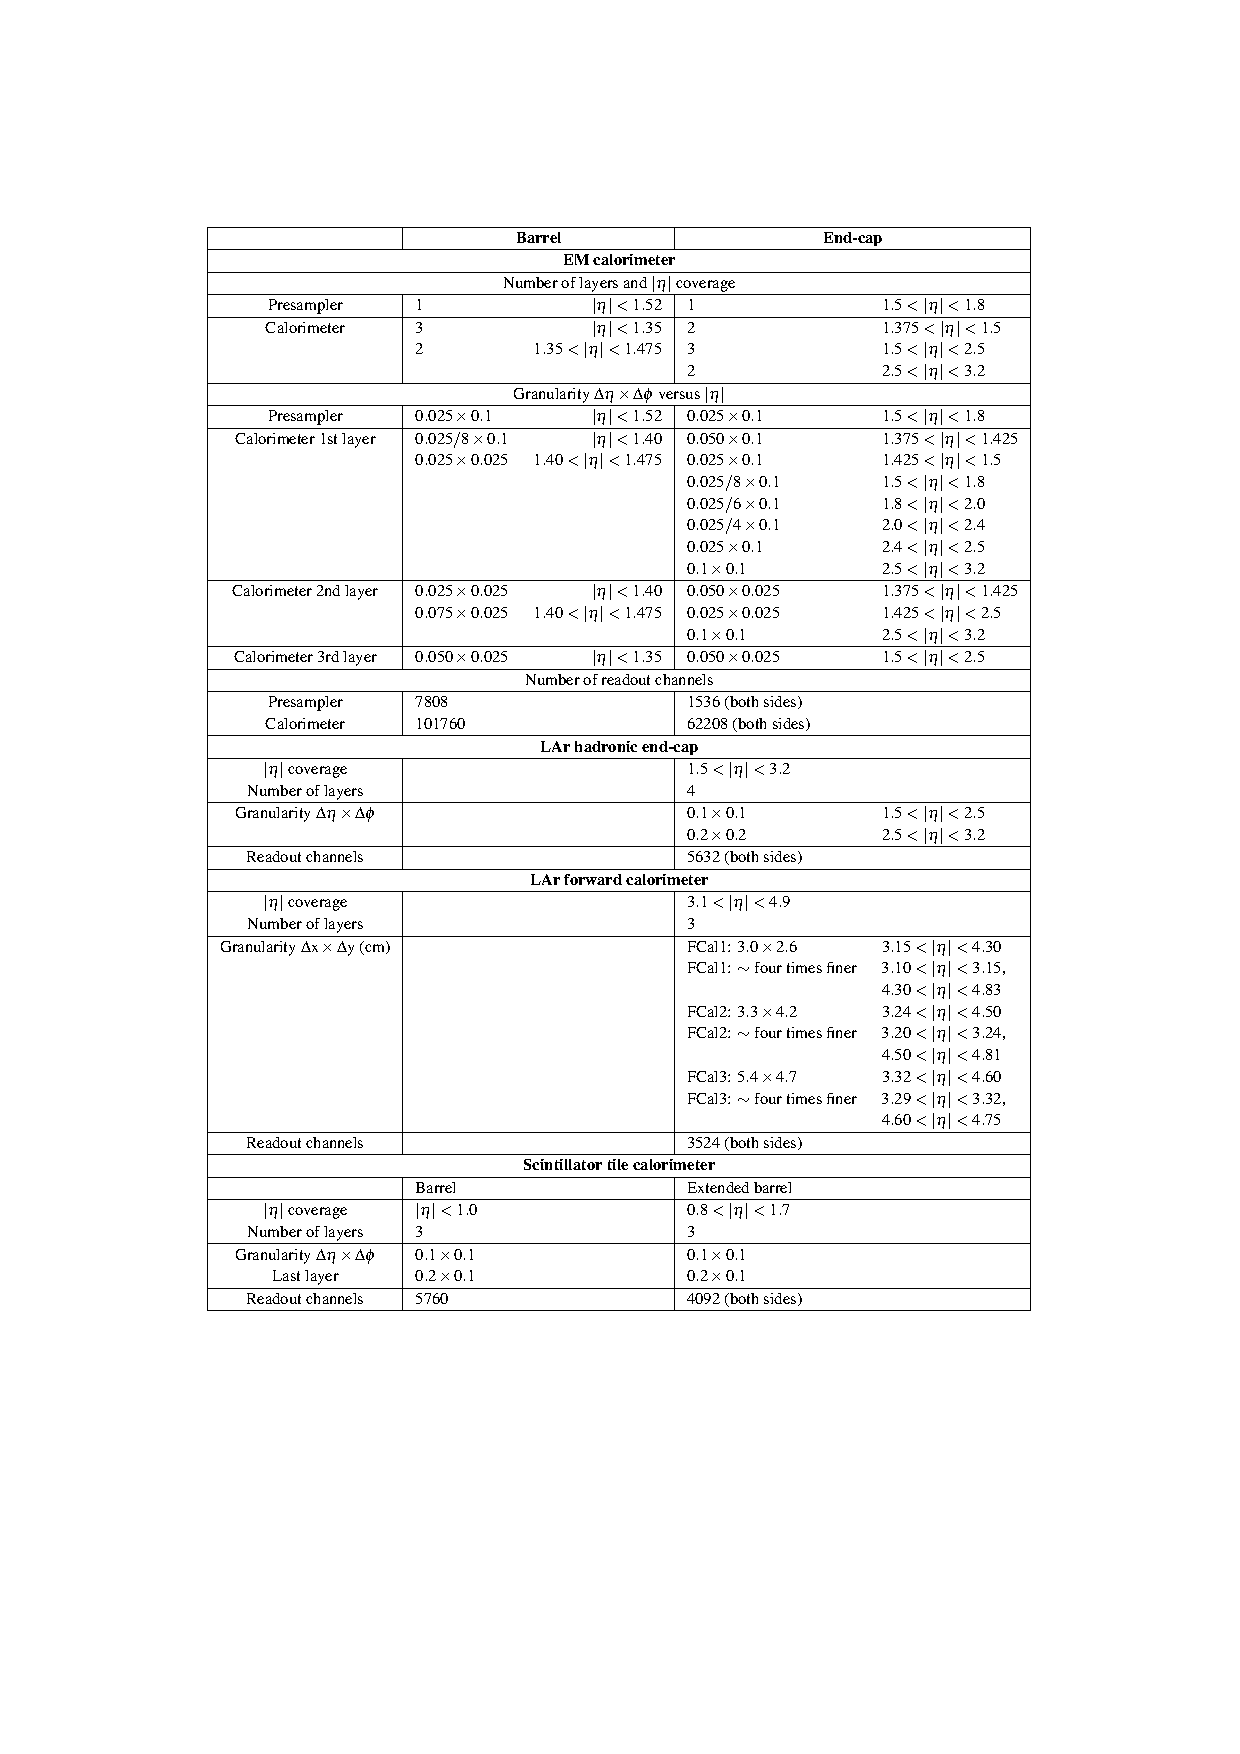
\includegraphics[width=1\linewidth, angle=0]{figs/Detector/tab_calo_granularity.pdf}
%  \end{center}
%  \caption[The key spatial coverage, granularity and readout parameters of the ATLAS calorimeter.]
%          {The key spatial coverage, granularity and readout parameters of the ATLAS calorimeter~\cite{det-ATLAS_Exp}.}
%  \label{tab:det-calo_granularity}
%\end{table}

Another important point about the ATLAS calorimeter is that it is a non-compensating calorimeter;
that is to say that the response of the detector to an electromagnetic particle (such as an electron)
is larger than the response of a hadronic particle (for example a pion).
This is because some energy is lost in hadronic cascade process;
mainly due to the energy required to release nucleons from calorimeter nuclei during spallation,
but also from the recoil energy given to the calorimeter nuclei
and neutrinos created during strong processes that can escape the calorimeter \cite{det-comp_calo, det-thesis_lene}.
The ATLAS calorimeter is initially calibrated to the EM-scale,
meaning that the inital energy measurement of a calorimeter assumes that the particle is only EM-interacting.
To account for the fact that the ATLAS calorimeter is non-compensation,
a jet energy scale correction is applied to a hadronic jet in the calibration processs,
which is described further in Section~\ref{sec:obj-jets_calib}.


\subsubsection{Energy Resolution of a Calorimeter}
\label{sec:det-calo_noise}

The energy resolution of a calorimeter is given by three terms:
\begin{equation}
  \left(\frac{\Delta E}{E}\right)^2 = \left(\frac{c_s}{\sqrt{E}}\right)^2 + \left(\frac{c_n}{\sqrt{E}}\right)^2 + c_c^2
\end{equation}

\noindent
The three terms are:
\begin{itemize}[leftmargin=*]
\item\textbf{Stochastic Term ($c_s$):}
  This term represent random fluctuations in the cascade shower process.
  This uncertainty is Poisson-like meaning that $\Delta E_s$ proportional to the square root of the number of photons/electrons,
  which gives us that $\Delta E_s \propto \sqrt{E}$. \vspace{0.5em}
\item\textbf{Noise Term ($c_n$):}
  This term represents effects that are independant of the energy measurement, such that $\Delta E_n = c_n$.
  Contributions to the noise term include electronic noise or radioactivity. \vspace{0.5em}
\item\textbf{Constant Term ($c_c$):}
  This term represents effects that are effect all energy measurements equally, such that $\Delta E_c/E = c_s$.
  Contributions to the constant term include regions of inactive material such as detector cracks and dead modules.
\end{itemize}

Approximate values of $c_s$ and $c_c$ for different components of the ATLAS calorimeter are given in Table~\ref{tab:det-calo_noise}.
The noise term depends strongly on $\eta$ and pile-up conditions so is not given.
For high-\pT{} objects ($\gt \sim 100$ GeV), such as the jets used in the di-$b$-jet searches, the constant term will become the dominant term,
as the other terms are supressed by the large values of $E$.

%{\renewcommand{\arraystretch}{1.2}
%\begin{table}[!htb]
%\centering
%\begin{tabular}{|c||c|c|c|}
%\hline
%Calorimeter Component  & Stochastic ($c_s$) [$\sqrt{\text{GeV}}$]  & Noise  ($c_n$) [GeV]        & Constant ($c_c$)  \\
%\hline
%EM Barrel              & 10\%                                  & $\sim$ 1\%-10\%                  & 0.7\%       \\
%EM End-cap             & 10\%                                  & $\sim$ 1\%-10\%                  & 0.7\%       \\
%Tile                   & 50\%                                  & $\sim$ 10\%-100\%                &   3\%       \\
%HEC                    & 50\%                                  & $\sim$ 10\%-100\%                &   3\%       \\
%FCAL                   & 100\%                                 & $\sim$ 10\%-100\%                &  10\%       \\
%\hline
%\end{tabular}
%\caption[A summary of the stochastic, noise and constant terms of the intrinsic energy resolution of components of the ATLAS calorimeter.]
%        {A summary of the stochastic, noise and constant terms of the intrinsic energy resolution of components of the ATLAS calorimeter.
%        The noise term depends on $\eta$ and pile-up conditions so only an approximate decade is given~\cite{det-ATLAS_Exp,det-thesis_lene}}
%\label{tab:det-calo_noise}
%\end{table}
%}


{\renewcommand{\arraystretch}{1.2}
\begin{table}[!htb]
\centering
\begin{tabular}{|c||c|c|c|}
\hline
Calorimeter Component  & Stochastic ($c_s$) [$\sqrt{\text{GeV}}$]   & Constant ($c_c$)  \\
\hline
EM Barrel              & 10\%                                       & 0.7\%       \\
EM End-cap             & 10\%                                       & 0.7\%       \\
Tile                   & 50\%                                       &   3\%       \\
HEC                    & 50\%                                       &   3\%       \\
FCAL                   & 100\%                                      &  10\%       \\
\hline
\end{tabular}
\caption[A summary of the stochastic and constant terms of the intrinsic energy resolution of components of the ATLAS calorimeter.]
        {A summary of the stochastic and constant terms of the intrinsic energy resolution of components of the ATLAS calorimeter~\cite{det-ATLAS_Exp}}
\label{tab:det-calo_noise}
\end{table}
}


\subsection{Muon Spectrometer}
\label{sec:det-MS}

The Muon Spectrometer (MS) is the outermost part of the ATLAS detector and is designed to detect charged particles pass through the calorimeters.
As the muon is the only particle detectable by the ATLAS detector that are not stopped by the calorimeter,
measurements in the Muon Spectrometer are used to identify muons.
The Muon Spectrometer consists of layers of detector detector providing positional measurements of 'hits'
in the prescence of a magenetic field, similar to the concept used for the Inner Detector (ID).
Furthermore, the position measurements from both the Muon Spectrometer and the ID are used to calculate the trajectory of the muon,
known as muon tracks, and from that the $p_T$ of the muon can be inferred.
By using position measurements from both the Muon Spectrometer and the ID, muon tracks have a long lever arm which improves momentum resolution.
Muon track reconstruction is further discussed in Section~\ref{sec:obj-leptons}.

In the barrel region ($|\eta| < 1.4$) the large barrel toroid provides the magnetic field,
in the end-cap region ($1.6 < |\eta| < 2.7$) the two smaller end-cap magnets  provide the magnetic field
and finally in the transition region ($1.4 < |\eta| < 1.6$) both sets of magnets contribute to the magnetic field.
A further description of the magnets used in ATLAS is found in the next section. 

Muon chambers are the detectors tasked with providing the muon position measurements required to reconstruct muon tracks.
In the barrel region,  muon chambers are arranged in three concentric cylindrical layers of chambers formed around the beam-pipe,
whilst in the transition and end-cap regions there are three layers of chambers either side of the barrel lying in disks perpendicular to the beam-pipe.

The muon chambers come in two types; trigger and precision.
The \textit{`trigger muon chambers'} provide a position measurement in 3-dimensions within 15--\SI{25}{\nano\second} which is used to identify muons tracks in the trigger.
The trigger muon chambers comprise of Resistive Plate Chambers (RPC’s) in the barrel 
and Thin Gap Chambers (TGC’s) in the end-cap regions.
Only measurements for $|\eta| < 2.0$ are used for triggering due to the high flux of muons close to the beam-pipe.
The \textit{`precision muon chambers'} provide a precise measurement of the muon position co-ordinates in the $R$-$z$ plane,
the plane in which track curvature occurs in the muon spectrometer, allowing for precise measurements of the muon track-$p_T$. 
In the region $|\eta| < 2.0$, the precision muon chambers are Monitored Drift Tubes (MDTs),
whilst at large pseudo-rapidities ($2.0 < |\eta| < 2.7$), Cathode Strip Chambers (CSCs) are used.
A schematic of the Muon Spectrometer is shown in Figure~\ref{fig:det-ms_schem}, the types of chambers used in each part is labelled.

There is an additional use of the muon spectrometer that relates to high-energy jets.
Whilst for most jets their shower is fully contained within the calorimeter
there are some jets, particularly at high-$p_T$, where a non-negligible fraction of energy from the shower goes beyond the calorimeter.
This effect, known as `punch-through', is estimated using energy deposits in the muon spectrometer.

\begin{figure}[!ht]
  \begin{center}
    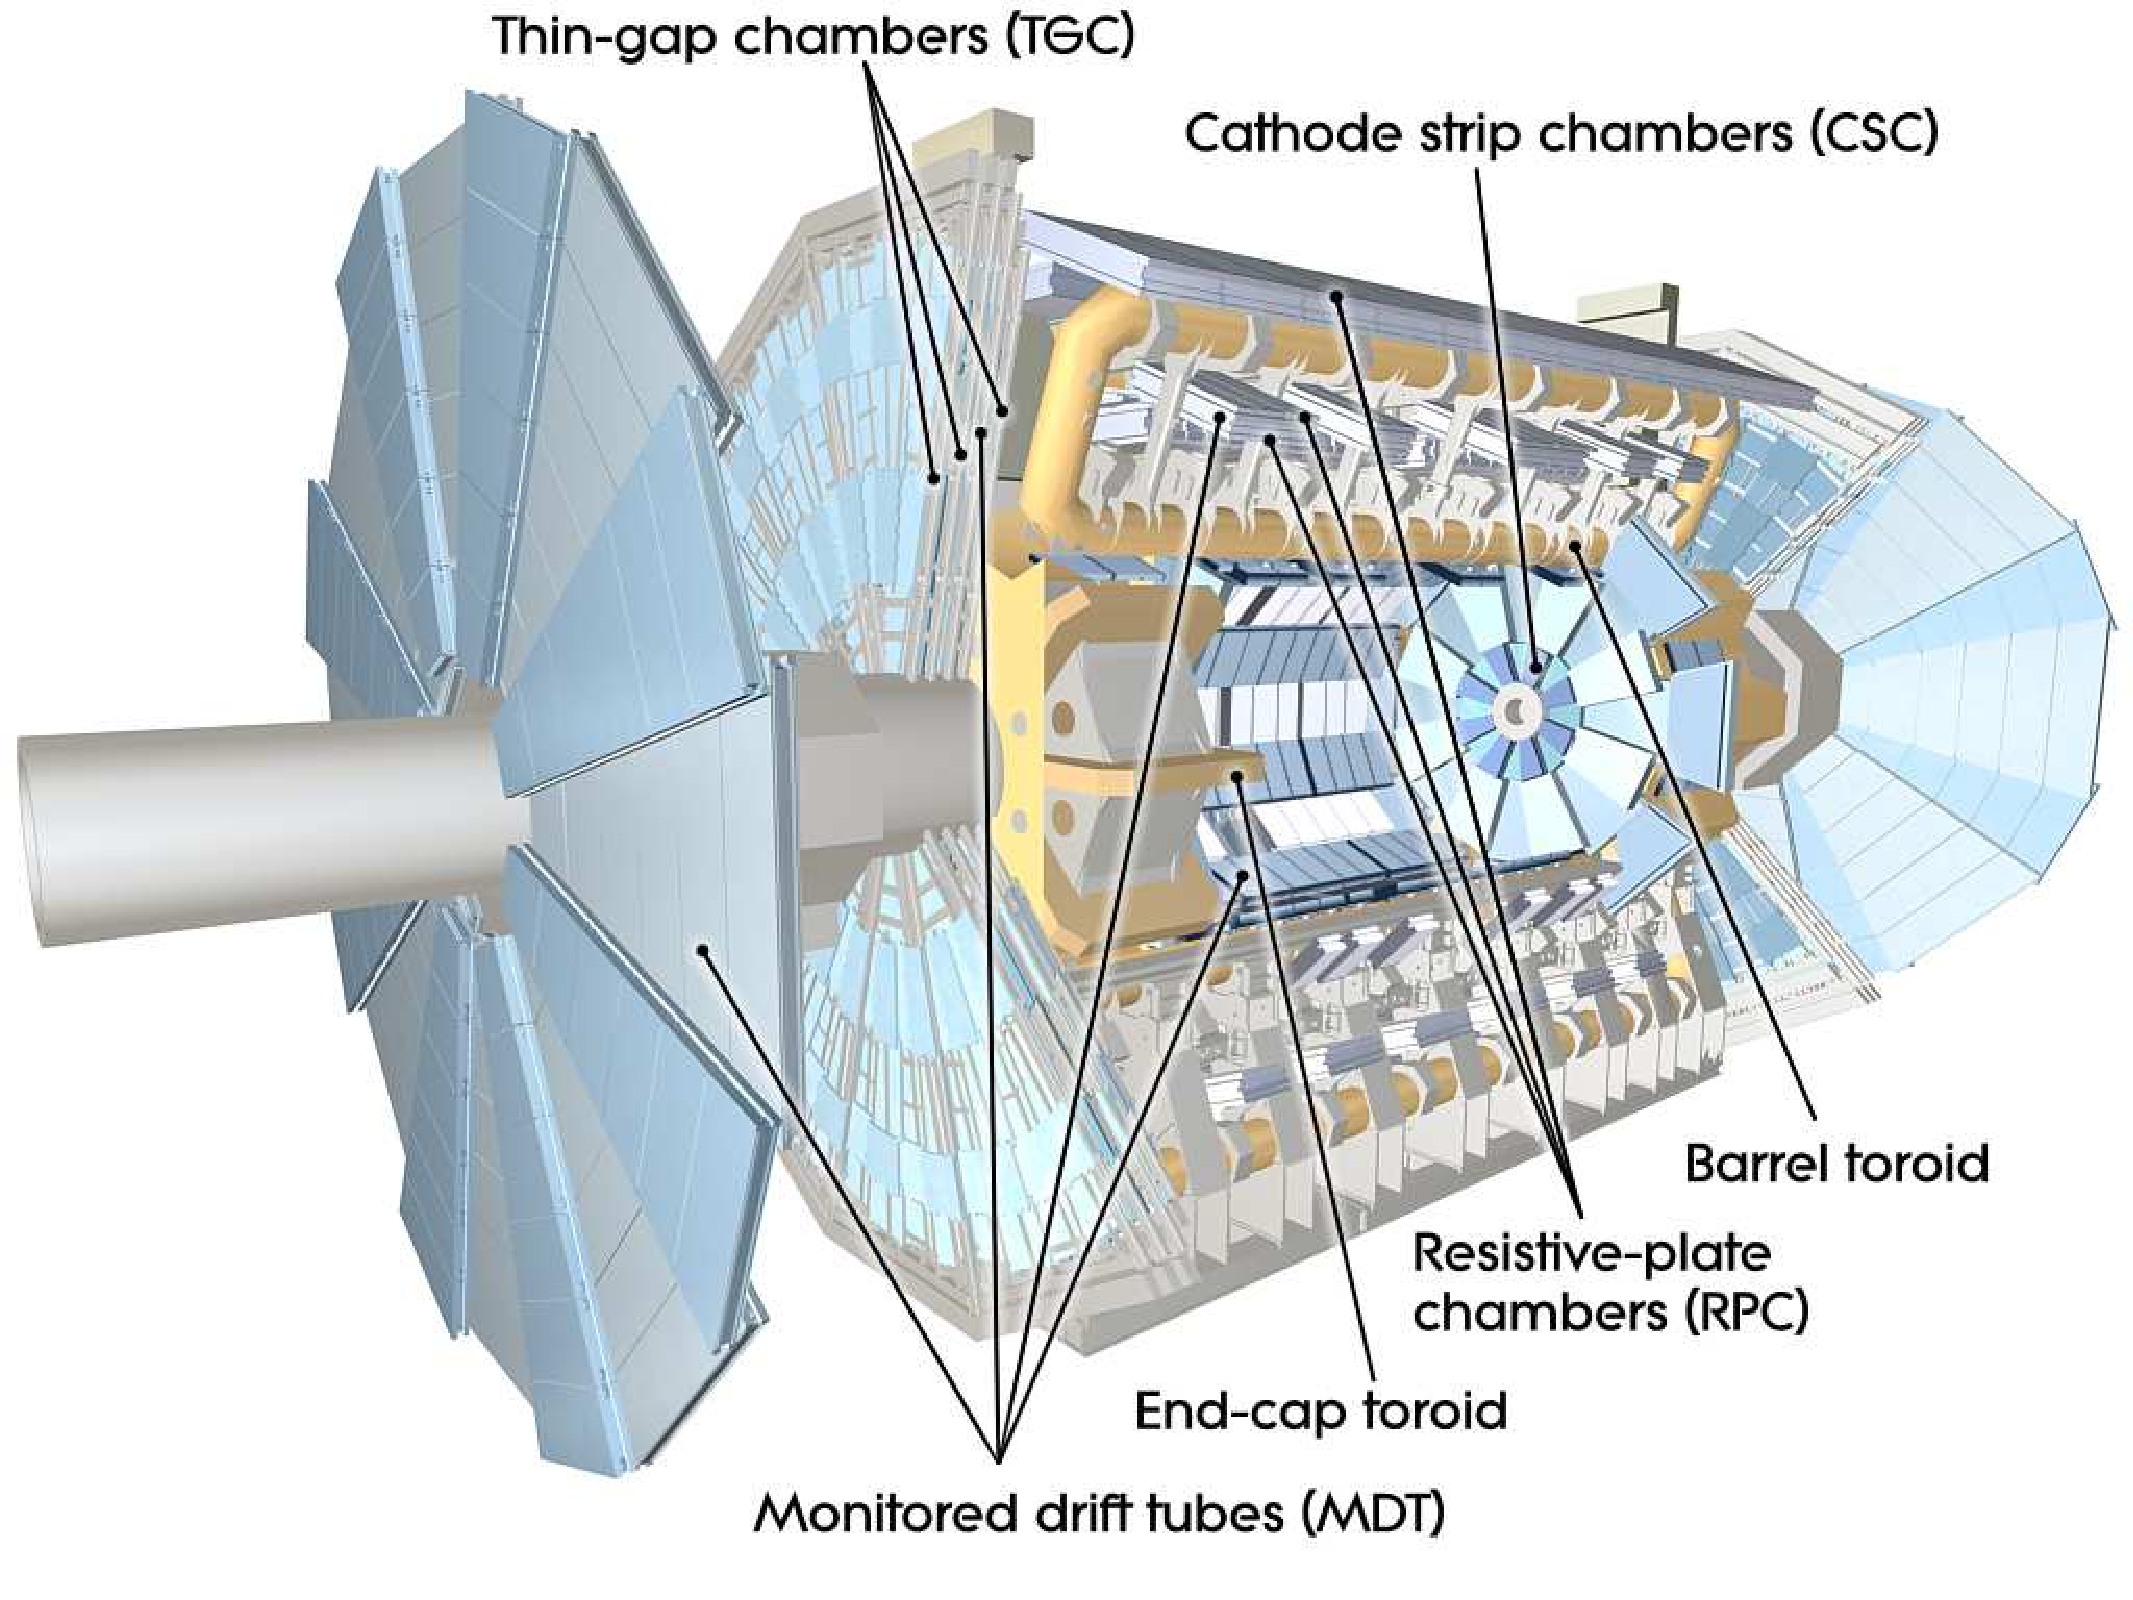
\includegraphics[width=0.8\linewidth, angle=0]{figs/Detector/MS_schem.pdf}
  \end{center}
  \caption[A cut-away of the ATLAS muon spectrometer.]
          {A cut-away of the ATLAS muon spectrometer (MS). The types of muon chamber used in each part of the MS are labelled on the figure.~\cite{det-ATLAS_Exp}.}
  \label{fig:det-ID_schem}
\end{figure}


\subsection{Magnets}
\label{sec:det-magnets}

\begin{figure}[!ht]
  \begin{center}
    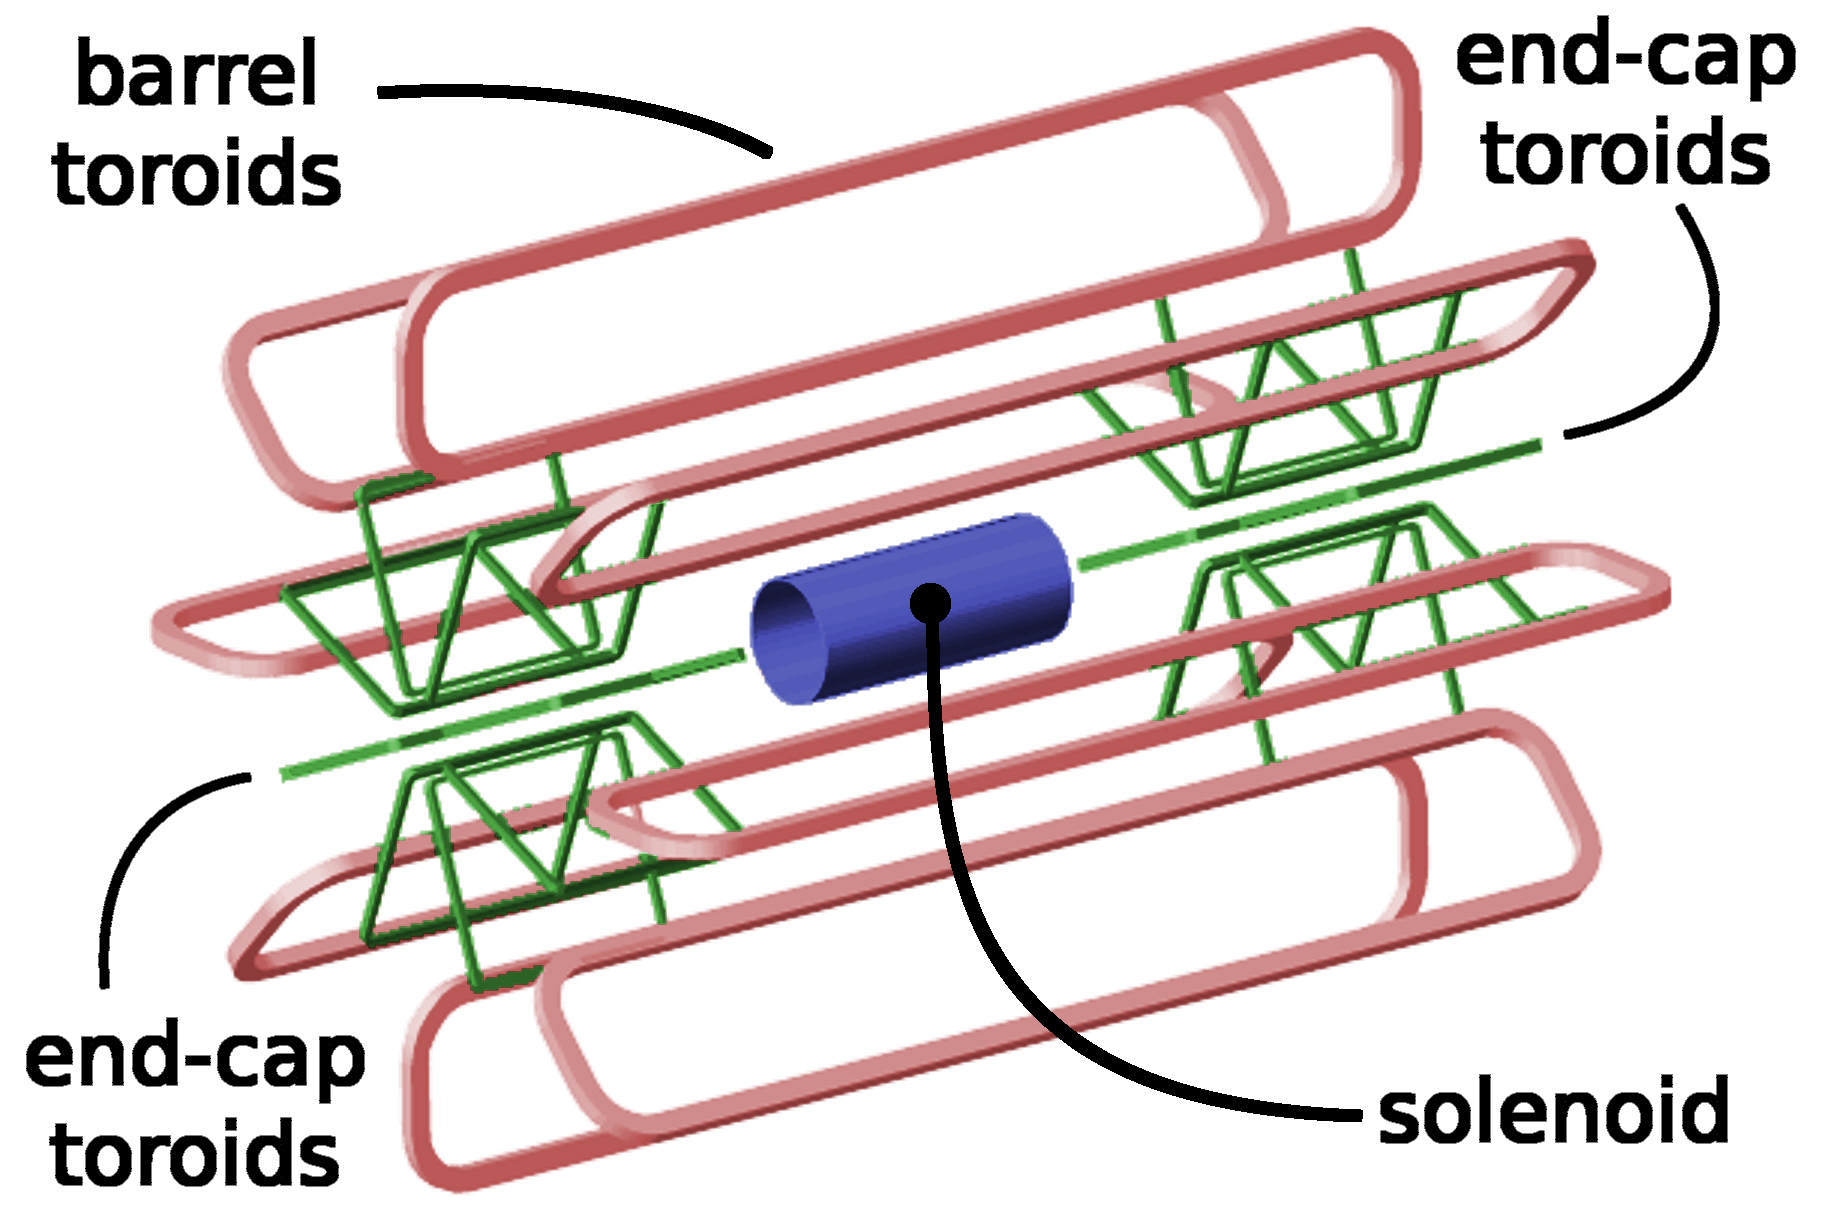
\includegraphics[width=1\linewidth, angle=0]{figs/Detector/Magnet_schem.png}
  \end{center}
  \caption[The layout of the ATLAS magnets.]{The layout of the ATLAS magnets~\cite{det-magnet_fig}.}
  \label{fig:det-magnet_schem}
\end{figure}


In ATLAS magnetic fields are important for obtaining the momentum and charge of particles from their observed trajectories in the ID and Muon Spectrometer.
ATLAS is made up of four large superconducting magnets;
the inner solenoid which surrounds the inner detector and provides a 2~T magnetic field within the ID.
The barrel toroid magnet provides a magnetic field of up to $\sim$0.5~T in the central regions of the muon spectrometer and
the two end-cap toroid magnets which produce a magnetic field of $\sim$1~T in the forward regions of the Muon Spectrometer.
Figure~\ref{fig:det-magnet_schem} shows the layout of the magnets in ATLAS~\cite{det-magnet_fig}.

\textbf{Note for AK: Trigger to be moved entirely to trigger chapter, reduces need for repetition.}

  
%%\section{Data Acquisition and Trigger}
%\section{Trigger}
%\label{sec:det-trig}
%
%In 2015 and 2016, the LHC has been colliding proton beams with a bunch spacing of \SI{25}{\nano\second},
%meaning that the ATLAS experiment has been taking data at a rate of 40 MHz.
%However, due to the large computing resources required to process and store each event,
%it is not possible to record all this data for use in an analysis.
%To resolve this problem,
%the ATLAS experiment uses a trigger system to reduce the event rate by
%selecting the events of interest that contain high-$p_{T}$
%%$\footnote{$p_{T}$ refers to the component of momentum transverse to the beam-line.} 
%physics objects, which indicate that a hard scatter has occurred in that event. 
%
%The ATLAS trigger-system has two levels;
%the first level trigger (L1) and the higher level trigger (HLT) \cite{det-run2_trigger}.
%Figure~\ref{fig:det-trigger_schem} shows a schematic outlining the trigger used in Run-2 \cite{det-run2_triggerPerf}. 
%
%\begin{figure}[!ht]
%  \begin{center}
%    \includegraphics[width=1\linewidth, angle=0]{figs/Detector/trigger_schem.png}
%  \end{center}
%  \caption[A schematic of the ATLAS trigger and data-acquisition system in Run-2, with a focus on the components required for triggering.]
%          {A schematic of the ATLAS trigger and data-acquisition system in Run-2, with a focus on the components required for triggering~\cite{det-run2_trigger}.}
%  \label{fig:det-trigger_schem}
%\end{figure}
%
%The first level trigger (L1) is hardware based which reduces the rate from 40~MHz to 100~kHz within a time window of \SI{2.2}{\micro\second}.
%The L1 trigger uses custom electronics to rapidly process information directly from the
%calorimeter and the muon spectrometer, searching for high-$p_{T}$ muon tracks and large calorimeter deposits.
%The information is then passed to the central trigger processor which uses a set of pre-defined conditions
%to decide if a L1 trigger accept is given and thus events are passed on to the next step of triggering.
%At the same time Regions of Interests (ROIs) are constructed around the objects that have fired the L1 trigger,
%which are passed on to the HLT. 
%
%The next step is the HLT, a software based trigger,
%which further reduces the event rate to 1~kHz within a time window of ~\SI{0.2}{\second}.
%The HLT uses the information from the full detector
%to perform a more complete reconstruction of the physics objects within the event,
%the most time consuming reconstruction algorithms only being run only within the ROIs taken from L1.
%The more complex event analysis allowed within the software-based trigger includes
%track reconstruction and therefore allows for $b$-jet identification.
%If the content of the event reconstruction passes a pre-set criteria, a HLT accept is issued
%meaning that the events are passed on for processing and storage. 
%% in offline computer farms (known as tier-0). 
%
%A further description of triggers used in the analysis,
%with a particular focus on the $b$-jet trigger performance
%is found in \ref{sec:bJetTrigger}\textit{(b-jet trigger chapter)}.
%
%
